\documentclass[crop,tikz]{standalone}% 'crop' is the default for v1.0, before it was 'previe
%\usetikzlibrary{...}% tikz package already loaded by 'tikz' option
\begin{document}
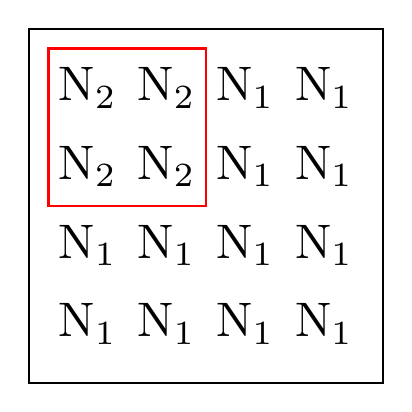
\begin{tikzpicture}[thick, every node/.style={scale=1.75}]
\draw[draw=black] (0.25,0.25) rectangle (4.75,4.75);
\draw[draw=red] (0.5,2.5) rectangle (2.5,4.5);
\node[] at (1, 4) {N$_{2}$}; \node[] at (2, 4) {N$_{2}$}; \node[] at (3, 4) {N$_{1}$};  \node[] at (4, 4) {N$_{1}$};
\node[] at (1, 3) {N$_{2}$}; \node[] at (2, 3) {N$_{2}$}; \node[] at (3, 3) {N$_{1}$};  \node[] at (4, 3) {N$_{1}$};
\node[] at (1, 2) {N$_{1}$}; \node[] at (2, 2) {N$_{1}$}; \node[] at (3, 2) {N$_{1}$};  \node[] at (4, 2) {N$_{1}$};
\node[] at (1, 1) {N$_{1}$}; \node[] at (2, 1) {N$_{1}$}; \node[] at (3, 1) {N$_{1}$};  \node[] at (4, 1) {N$_{1}$};

\end{tikzpicture}

\end{document}